\documentclass[12pt,twocolumn]{article}
% Required packages


\usepackage[utf8]{inputenc}
\usepackage[margin=1in]{geometry}
\usepackage{setspace}
\usepackage{graphicx}
\usepackage{epstopdf}
\usepackage{amsmath}
\usepackage{amssymb}
\usepackage[numbers]{natbib}
\usepackage{booktabs}
\usepackage{subcaption}

\usepackage{braket}
\usepackage{enumitem}
\usepackage{pifont}
\usepackage{hyperref}
\usepackage{newunicodechar}
\newunicodechar{ }{~}
\usepackage{array}
\usepackage{tabularx}
\usepackage{algorithm}
\usepackage{algpseudocode}

% Double spacing as required
\doublespacing

% Title and author information
\title{Quantum Synthetic Data Generation for Industrial Bioprocess Monitoring}

\author{
Shawn M. Gibford\textsuperscript{1}, Mohammad Reza Boskabadi\textsuperscript{1},\\ Christopher J. Savoie\textsuperscript{2}, Seyed Soheil Mansouri\textsuperscript{1}\\
\textsuperscript{1}Dept. Chemical and Biochemical Engineering, \\
Technical University of Denmark,
Kongens Lyngby, Denmark\\
\textsuperscript{2}SiC Systems Inc., Franklin, TN, USA
}

\date{} % Leave empty for submission

\begin{document}

\maketitle
% Abstract section (max 150 words)
\begin{abstract}
\noindent
Data scarcity in biomanufacturing poses challenges for model development, process monitoring, and optimization. We propose a Quantum Wasserstein Generative Adversarial Network with Gradient Penalty (QWGAN-GP) to generate synthetic time series data for laboratory-scale bioprocesses. The generator employs a Parameterized Quantum Circuit (PQC), with the aim of reducing dependence on scarce experimental data. Under a matched parameter budget and matched training epochs, the quantum generator reproduces the temporal dynamics of the optical density series within the evaluated metrics, at a fidelity comparable to size-matched classical baselines, focusing on optical density as a key measurement for dry biomass estimation. These results provide a proof-of-concept for quantum-enhanced synthetic data generation in bioprocess engineering, with potential downstream applications in soft sensor development and predictive control.
\end{abstract}

% Topical Heading and Keywords
\noindent\textbf{Topical Heading:} Process Systems Engineering

\noindent\textbf{Keywords:} quantum machine learning, Generative adversarial network, Bioprocess monitoring, Synthetic time series generation, Data augmentation

% Plain Language Summary (max 250 characters)
\section*{Plain Language Summary}
We developed a quantum computing method to create realistic artificial data for biomanufacturing processes. This helps overcome data shortages and improves process control and monitoring in industrial biotechnology applications.

\section{Introduction}

\begin{figure*}
    \centering
    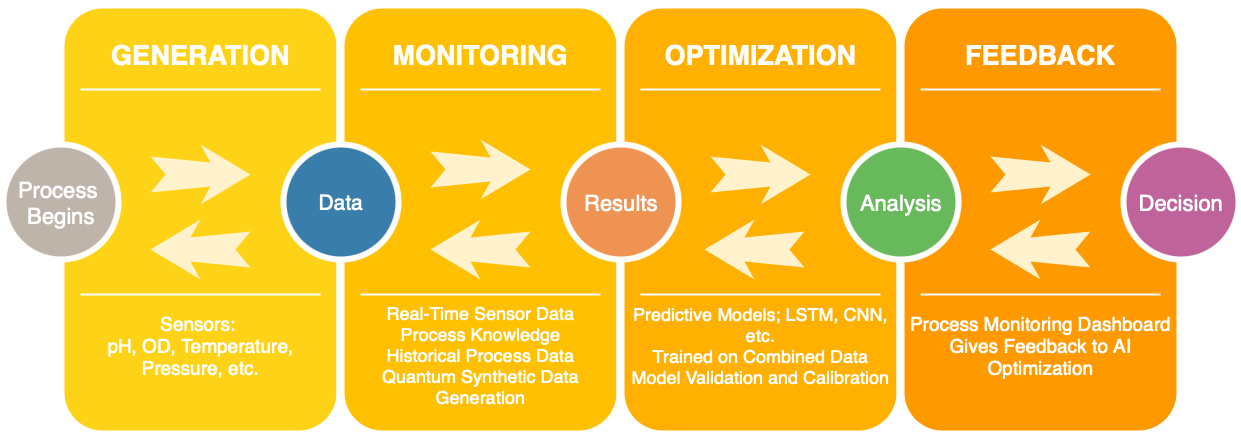
\includegraphics[height = 7cm, width = 17cm]{concept_diagram.png}
    \caption{Conceptual diagram of how we envision using quantum generative AI within industrial bioprocess engineering.}
    \label{fig:concept_diagram}
\end{figure*}

Machine Learning (ML) and Artificial Intelligence (AI) have emerged as transformative tools in diverse scientific disciplines, from cancer research to financial analysis (Figure~\ref{fig:concept_diagram}). \cite{clinical_iqbal_2021} \cite{vakili2024quantumcomputingenhancedalgorithmunveils} \cite{artificial_ahmed_2022} \cite{Orus2019QuantumCF}  However, complex systems such as manufacturing, drug discovery, and formulated products \cite{emerson2021} have lagged in fully embracing ML/AI methodologies compared to other fields. This discrepancy reflects unique challenges including high dimensionality, inherent variability, and complex underlying chemical, physical, or biological mechanisms. \cite{boskabadi2025virtual}

Bioprocess engineering exemplifies these challenges. The field is crucial for producing biofuels, pharmaceuticals, and sustainable materials, yet data analytics applications often grapple with limited datasets due to time-consuming and expensive experiments. \cite{stoneOptimize} This scarcity hinders development of accurate predictive models, particularly for hard-to-quantify quality indicator variables (QIVs) essential for process optimization and real-time monitoring.

Critical QIVs in bioprocesses include biomass concentration, which is often estimated through optical density measurements or viable cell counts but requires complex calibration and suffers from interference in high-density cultures. \cite{kiviharju2008biomass} Product concentration and quality, such as monoclonal antibody titers and glycosylation patterns in mammalian cell culture, typically require offline analytical methods such as High-Performance Liquid Chromatography (HPLC) or mass spectrometry. Metabolic activity indicators, including specific growth rates, substrate consumption rates, and metabolic flux distributions, are fundamental QIVs that are difficult to quantify in real-time without sophisticated analytical platforms. The integration of ML with bioprocess engineering has been gradually expanding, with applications spanning process monitoring, \cite{peng2025machinelearningmethodssmall} optimization, \cite{sharma2025ai} and control. \cite{mondal2023review} These approaches have demonstrated potential to address limitations of traditional mechanistic models, particularly when dealing with non-linear dynamics and multivariate nature of biological systems.

\subsection{Data Scarcity as a Fundamental Limitation}

A fundamental challenge limiting widespread adoption of machine learning in bioprocess engineering is data scarcity. \cite{lim2023opportunities, duongtrung2023when} Unlike fields such as computer vision or natural language processing, where datasets may be comprised of millions of samples, bioprocess datasets are typically constrained by several factors. Bioprocess experiments, particularly on pilot and production scales, involve substantial costs in terms of equipment, raw materials, personnel, and time.  \cite{shariatifar2025digital} \cite{exploring_hernndezromero_2025} A single bioreactor run at pilot or production scale may take weeks to complete and can be costly, often on the order of several hundreds of thousands of dollars or more, severely limiting the number of experimental conditions that can be feasibly explored. \cite{exploring_hernndezromero_2025} Biological systems exhibit inherent stochasticity and sensitivity to environmental conditions, resulting in significant batch-to-batch variability even under nominally identical operating conditions. Commercial bioprocesses represent significant intellectual property, which results in limited data sharing across the industry. While fields such as computer vision benefit from open datasets with millions of examples, bioprocess data typically remains siloed within individual companies or research groups. These factors collectively result in datasets that are often too small to effectively train complex ML models, particularly deep learning architectures that typically require substantial amounts of diverse training data.

\subsection{Synthetic Data Generation Approaches}

Synthetic data generation is a promising approach to address data scarcity challenges in bioprocess engineering. \cite{liu2024bestpracticeslessonslearned} By creating artificial datasets that faithfully represent statistical properties and dynamic behaviors of real bioprocesses, synthetic data approaches can potentially overcome limitations in data availability while avoiding confidentiality concerns (a comparison of approaches is provided in Supplementary Table A1 %~\ref{tbl:bioprocess_methods}).

First-principles models have been used to simulate bioprocess dynamics under various conditions, generating synthetic time series data. \cite{vidossich2021role}  Although this approach ensures physical consistency, its fidelity is limited by the accuracy of the underlying model and its ability to capture process variability and uncertainty. Methods such as Gaussian process regression \cite{rasmussen2006gaussian} and multivariate statistical models can generate synthetic data based on estimated probability distributions. These approaches excel at reproducing statistical properties, but often struggle to capture complex temporal dependencies and rare events.

Machine learning models such as variational autoencoders (VAEs) and generative adversarial networks (GANs), including time-series-specific architectures \cite{yoon2019TimeGAN}, can learn directly from available data to generate synthetic samples.  \cite{akkem2024comprehensive} These approaches offer flexibility in generating diverse datasets without requiring detailed mechanistic understanding, although their performance is highly dependent on the quality and quantity of training data. Combining mechanistic knowledge with data-driven techniques represents a promising direction for generation of synthetic bioprocess data.

Despite these advances, significant challenges remain in generation of high-quality data: accurate capture of complex temporal dependencies, incorporation of mechanistic knowledge constraints, ensuring physical realizability, and validating the quality of synthetic data. Addressing these challenges requires novel methodological approaches. These limitations motivate exploring alternative computational paradigms, including quantum approaches, which \emph{may} offer advantages for certain structured learning tasks in chemical and biochemical engineering \cite{bernal2022perspectives}.

\subsection{Quantum Generative Adversarial Networks}

Quantum Generative Adversarial Networks (QGANs) embed Parameterized Quantum Circuits within the generator of a GAN \cite{Dallaire_Demers_2018, Lloyd_2018, Zoufal_2019}. This motivates the falsifiable question that frames the present study: \emph{can a PQC generator, operating in an exponentially large Hilbert space with $\mathcal{O}(\mathrm{poly}(n))$ parameters, match or exceed a classical generator of equivalent parameter count on a low-data bioprocess task?} Prior work has reported QGAN results in low-data regimes and on multimodal distributions \cite{rudolph2022generationhighresolutionhandwrittendigits, he2025qganbaseddataaugmentationhybrid}, with applications in finance \cite{orlandi2024enhancing} and optimization \cite{Mugel2022}; GANs more broadly, including classical recurrent variants, have also been applied to healthcare time series \cite{esteban2017realvaluedmedicaltimeseries}. We test this claim directly under a matched-parameter, matched-epoch protocol. Current quantum hardware constraints, noise, decoherence, and limited circuit depth, restrict practical scalability \cite{Cerezo_2021}, but QGANs offer a candidate alternative when classical GANs struggle with intricate temporal dependencies in limited datasets \cite{goodfellow2014generativeadversarialnetworks, lloyd2013quantumalgorithmssupervisedunsupervised}. A detailed review of QGANs and their relationship to classical GANs is provided in Section~2.


\subsection{Principal Contributions}

The principal contributions of this work are:

- Matched-Parameter Comparison Protocol: A parameter-matched, matched-epoch, multi-seed protocol for comparing a PQC generator against size-matched classical baselines on a data-scarce bioprocess task.

- QWGAN-GP for Process Data Synthesis: A hybrid QWGAN-GP architecture, with a Parameterized Quantum Circuit generator and a classical critic, applied to laboratory-scale bioprocess time series.

- Empirical Evaluation on a Photobioreactor Campaign: A quantitative evaluation on a single real-world cultivation dataset, reporting fidelity comparable to classical baselines under the matched protocol rather than a demonstrated quantum advantage.

- Open Science and Reproducibility: We make our code and datasets publicly available, facilitating independent verification and future advances in quantum-enhanced bioprocess engineering.

A decision-driven workflow is also outlined in the Outlook as an organising concept for future closed-loop deployment; it is not an empirical contribution of this study.

The remainder of this paper is structured as follows. Section~2 reviews classical and quantum machine learning foundations. Section~3 describes the QWGAN-GP architecture and the photobioreactor experimental setup. Section~4 presents results, key contributions, and discusses implications and limitations. Section~5 offers concluding remarks.

\section{Classical and Quantum Machine Learning}


This section reviews the classical and quantum machine learning foundations underpinning our approach, beginning with GANs and the WGAN-GP formulation before turning to quantum machine learning and QGANs.


\subsection{Generative Adversarial Networks and WGAN-GP}

GANs represent the foundation of modern synthetic data generation. \cite{goodfellow2014generativeadversarialnetworks} The GAN framework (illustrated in Supplementary Figure A1 %~\ref{fig:classical_gan}) 
consists of two neural networks engaged in a competitive minimax game: a generator G that learns to produce synthetic data, and a discriminator D that distinguishes between real and synthetic samples. The objective function is formulated as:



\begin{multline}
\min_G \max_D V(D,G) = \mathbb{E}_{x\sim p_{data}(x)}[\log D(x)] \\
+ \, \mathbb{E}_{z\sim p_z(z)}[\log(1-D(G(z)))]
\end{multline}

where $p_{data}(x)$ represents the real data distribution and $p_z(z)$ is the noise distribution.

For time-series applications, specialized architectures such as TimeGAN \cite{yoon2019TimeGAN} incorporate recurrent components to better capture temporal dependencies. However, classical GANs remain constrained by training stability issues, limited ability to capture multimodal distributions, and sensitivity to hyperparameter selection \cite{Arjovsky2017, gulrajani2017improved}, limitations that become pronounced with the small datasets typical of bioprocess engineering.

Despite their success, the original GAN formulation suffers from mode collapse and vanishing gradients \cite{Arjovsky2017}. The Wasserstein GAN (WGAN) addressed these instabilities by replacing the Jensen--Shannon divergence with the Earth Mover's distance \cite{arjovsky17a}, but its reliance on weight clipping introduced pathological behavior. The Wasserstein GAN with Gradient Penalty (WGAN-GP) \cite{gulrajani2017improved} refined this by imposing a soft gradient constraint:

\begin{equation}
\label{eq:wgangp}
\begin{split}
\min_G \max_D \bigl[ & \mathbb{E}_{x\sim P_r}[D(x)] - \mathbb{E}_{z\sim P_z}[D(G(z))] \\
& - \lambda\mathbb{E}_{\hat{x}\sim P_{\hat{x}}}\bigl[(\|\nabla_{\hat{x}}D(\hat{x})\|_2 - 1)^2\bigr] \bigr]
\end{split}
\end{equation}


The WGAN-GP framework employs a critic network D(·) and generator network G(·) in a minimax optimization scheme. The objective approximates the Wasserstein distance between the real data distribution $P_r$ and the distribution of generated samples produced from noise distribution $P_z$. To enforce the Lipschitz constraint, a gradient penalty term is introduced with coefficient $\lambda $(typically set to 10), which operates on interpolated samples $\hat{x} = \epsilon x + (1-\epsilon)G(z)$ where $\epsilon \sim \text{Uniform}(0,1)$. These interpolated points, distributed according to $P_{\hat{x}}$, provide a differentiable path between real and generated samples, enabling stable enforcement of the 1-Lipschitz continuity requirement without weight clipping.

This solution stabilizes training across architectures and mitigates issues with weight clipping, leading to improved sample quality and more reliable convergence \cite{villani2008optimal}. A detailed mathematical derivation of the Wasserstein distance and the Kantorovich--Rubinstein duality is provided in Supplementary Section~A.2.2.

\subsection{Quantum Machine Learning and QGANs}

Quantum machine learning (QML) leverages quantum mechanical principles to improve learning algorithms, with recent advances demonstrating potential advantages in expressivity, training efficiency, and generalization \cite{Biamonte2017, kashyap2025advancesmachinelearningquantum}. Relevant approaches include quantum-enhanced sampling, quantum kernels \cite{havlicek2019supervised, schuld2019quantum}, and variational quantum algorithms, each offering potential benefits for data-scarce bioprocess applications \cite{Cerezo_2021}.


QGANs are a hybrid quantum-classical approach in which a Parameterized Quantum Circuit (PQC) serves as the generator, first introduced by Dallaire-Demers and Killoran \cite{Dallaire_Demers_2018}. Superposition and entanglement give a PQC access to a state space that grows exponentially with qubit count; whether this translates into a practical advantage over a parameter-matched classical generator is an empirical question that remains open and is one we examine directly in this work rather than assume \cite{rudolph2022generationhighresolutionhandwrittendigits}. QGANs have been applied to finance \cite{orlandi2024enhancing} and optimization \cite{Mugel2022}; classical recurrent GAN variants have also been applied to healthcare time series \cite{esteban2017realvaluedmedicaltimeseries}. For time-series generation, models such as TimeGAN \cite{yoon2019TimeGAN} and DoppelGANger \cite{Lin_2020} have shown strong classical performance, but remain limited by computational constraints with high-dimensional distributions, a gap that quantum approaches may help address.

\section{Methods}

\subsection{QWGAN-GP Architecture Overview}

Our QWGAN-GP employs a hybrid quantum-classical architecture in which the generator
is a Parameterized Quantum Circuit (PQC) and the critic is a classical convolutional
neural network trained under the WGAN-GP objective (Eq.~\ref{eq:wgangp}). The quantum
generator uses 5 qubits arranged in three layers, incorporating Hadamard gates for
superposition, IQP encoding with parameterized $R_z$ rotations, two strongly entangling
layers with $\text{Rot}(\phi, \theta, \omega)$ gates, and range-based CNOT gates for
entanglement. The circuit outputs 10-dimensional samples via Pauli-X and Pauli-Z
expectation values, matching the rolling window subsequence length. The generator
contains 55 trainable parameters. Full circuit specifications and the critic architecture
are detailed in Supplementary Sections A.5 and A.8, respectively (see also Figure A4).%~\ref{fig:quantum_circuit}).

The raw optical density time series was transformed to log returns, normalized to zero
mean and unit variance, and passed through an inverse Lambert W transform to reduce
heavy-tailed characteristics prior to training (details in Supplementary Section A.7).
Overlapping subsequences of length 10 with stride 2 were extracted using a rolling
window approach \cite{dimoudis2023utilizing}.  % [41] removed: it was adaptive rolling-median anomaly detection, not subsequence extraction (R1-m1)

The WGAN-GP loss formulation (Eq.~\ref{eq:wgangp}) was chosen for the quantum generator because it provides stable gradients and meaningful convergence metrics, and mitigates mode collapse issues that can be exacerbated by the discrete nature of quantum measurements; we do not attribute reduced mode collapse to the quantum generator.

\subsection{Circuit Design Rationale}

The generator circuit was fixed by three deliberate design choices, each
constrained by the matched-parameter, low-data setting of this study.

\textbf{Qubit count.} The generator uses 5 qubits. The qubit count is
dictated by the rolling-window length: each length-10 subsequence is produced
from Pauli-X and Pauli-Z expectation values over the 5-qubit register
($5$ qubits $\times\,2$ observables $=10$ outputs), so the window length and
qubit count are coupled by construction rather than tuned independently. Five
qubits give a $2^{5}$-dimensional state space, which is more than sufficient
to embed a length-10 log-return window while keeping the parameterised circuit
trainable by exact backpropagation on a state-vector simulator at the data
scale available here. The locked configuration therefore has 5 qubits,
3 layers, and 55 trainable parameters, decomposed as one IQP-encoding
parameter per qubit plus 3 strongly-entangling rotation parameters per qubit
per layer.

\textbf{Ansatz expressibility versus trainability.} The reported circuit
(IQP encoding $+$ strongly-entangling layers, range entangler, 55 parameters)
was selected against a multi-seed ansatz comparison at a matched 2000-epoch
budget. We compared three alternatives at increased capacity or different
connectivity: a depth-4 range-entangled circuit (75 parameters), a depth-8
range-entangled circuit (135 parameters), and a depth-4 linear-entangled
circuit (75 parameters), each over 5 seeds. Increasing parameter count and
circuit depth, or changing the entangler topology, did \emph{not} yield a
fidelity improvement over the compact 55-parameter circuit at the matched
budget on this dataset (per-model values reported in Section~4 and the
supplementary figure suite). Consistent with the expressibility--trainability
tradeoff for variational circuits, the deeper/larger ansatz is harder to
optimise in the low-data, fixed-epoch regime without a corresponding accuracy
gain, motivating the choice of the smaller circuit as the reported
configuration.

\textbf{Classical critic with a quantum generator.} The critic is a classical
convolutional network and only the generator is quantum. This is deliberate:
the WGAN-GP objective requires a gradient penalty on interpolated samples,
which is cheap and stable to evaluate with a classical critic, whereas placing
the discriminator on the quantum device would add measurement-shot noise to
the critic gradient and substantially increase circuit evaluations per step
without benefiting the quantity of interest (the generated distribution). A
classical critic also makes the comparison against the matched classical
WGAN-GP baselines clean: the only component that differs between the quantum
and classical entrants is the generator, isolating the effect of the quantum
circuit.

\subsection{Photobioreactor Experimental Setup}

Time-series data were collected from a 20-liter photobioreactor (LUCY\textregistered, Synoxis Algae) designed for laboratory- and pilot-scale cultivation of microalgae; the system is also available in a larger 300-liter configuration. The 20-liter unit used in this study is shown schematically in Figure~\ref{fig:lucy}. The system comprises six vertical borosilicate glass tubes (6~cm OD, 120~cm length) connected in parallel, with SALT technology (spiral air lift tubular circulation) for gentle mixing, controlled aeration, and programmable lighting managed by an integrated automated controller.  

The system continuously monitors pH, temperature, optical density, dissolved oxygen, and pressure via feedback control loops, with data logged at 10-minute intervals by an internal data acquisition system. The OD sensor operates at 880~nm and reports values in arbitrary units based on logarithmic attenuation, calibrated against fresh culture medium.

\paragraph{Dataset and preprocessing.}
The study uses a single LUCY photobioreactor cultivation campaign
% source: revision/results/model_info.json#dataset.independent_campaigns (=1)
% source: revision/results/model_info.json#dataset.raw_csv_rows (=778)
comprising 778 raw optical-density time points logged at 10-minute intervals.
% source: revision/results/model_info.json#dataset.log_return_rows (=777)
First differencing into log-returns yields 777 log-return observations
($r_t = \ln \mathrm{OD}_t - \ln \mathrm{OD}_{t-1}$), which are standardized to
zero mean and unit variance, passed through an inverse Lambert~$W$ heavy-tail
correction, and rescaled to $[-1, 1]$.
% source: revision/results/model_info.json#dataset.window_length (=10)
% source: revision/results/model_info.json#dataset.window_stride (=2)
% source: revision/results/model_info.json#dataset.rolling_windows (=384)
Overlapping subsequences of length 10 with stride 2 are then extracted with a
rolling window, producing 384 training windows.
% source: revision/results/model_info.json#dataset.train_windows (=384)
% source: revision/results/model_info.json#dataset.val_windows (=0)
% source: revision/results/model_info.json#dataset.test_windows (=0)
Because only one independent campaign is available, all 384 windows are used for
training; no held-out validation or test split is carved out, as a 384-window
single campaign is too small to support a held-out split without severely
under-powering training (stated openly per the calibration-honesty standard,
R1-M5). Multi-campaign generalization is identified as future work.
% source: revision/results/model_info.json#seed_set ([42,43,44,45,46])
All reported quantitative results are aggregated over 5 independent random
seeds (42, 43, 44, 45, 46) and reported as mean $\pm$ standard deviation.


\section{Results and Discussion}

\subsection{Results}

We evaluate the fidelity of the generated synthetic time series using four complementary metrics. Dynamic Time Warping (DTW) distance measures temporal alignment, capturing non-linear dependencies where process variations cause phase shifts in growth events. Probability density and cumulative distribution functions assess distributional fidelity. Quantile--quantile plots evaluate tail behavior. Autocorrelation functions verify that no spurious temporal structure is introduced. Together, these metrics cover the statistical properties most critical for downstream bioprocess modeling applications.

\paragraph{Evaluation scale.}
Every fidelity metric is reported on \emph{both} the transformed log-return
scale (the space the generator is trained in) and the original optical-density
(OD) scale (obtained by inverting the preprocessing pipeline), so that the
physical-unit fidelity is explicit (R1-m3). Table~\ref{tbl:eval_scale} states
the scale of each metric family and the headline 55-parameter IQP:SEL quantum
generator value on each scale.

\begin{table}[h]
\centering
\caption{Evaluation metrics and the scale on which each is computed. Values are
for the 55-parameter IQP:SEL quantum generator, Pipeline~B (native
preprocessing), representative seed.}
\label{tbl:eval_scale}
\small
\begin{tabular}{@{}lccc@{}}
\toprule
\textbf{Metric} & \textbf{Transformed (log-return)} & \textbf{Original (OD)} & \textbf{Reported on} \\
\midrule
EMD                 & 0.1209437521974767 & 0.022937980562900886 & both scales \\
DTW (mean)          & 0.9343404967853801 & 0.2648187239898106   & both scales \\
Moment: mean        & 0.1232816505352802 & 1.4070339987298917   & both scales \\
Moment: std         & 0.07206523080095577 & 0.8839933147241738  & both scales \\
Moment: skewness    & -0.03262545792264619 & 1.3655798412279025 & both scales \\
Moment: kurtosis    & -0.08214151764010014 & 0.7768219209344931 & both scales \\
ACF (lag~1, mean)   & -0.0814285239177223 & 0.6965233188661055  & both scales \\
\bottomrule
\end{tabular}
\end{table}

PDF/CDF, Q--Q, and ACF diagnostic plots in the main text are shown on the
transformed log-return scale (the training space); the corresponding
original-OD-scale versions are provided as regenerated figures
(\texttt{revision/results/figures/acf\_iqp\_sel\_55\_repro}, dual-scale). DTW,
EMD, and the distributional moments are reported on both scales as above.

\textbf{Dynamic Time Warping.}
Under the matched parameter budget and matched 2000-epoch training contract,
the OD-scale DTW distance between original and synthetic sequences for the
55-parameter IQP:SEL quantum generator was approximately 0.30 (mean over 5
seeds; Figure~\ref{fig:DTWD}). An earlier frozen pre-v1.0 best-case checkpoint
reported a DTW distance of 0.6843; that value was not re-emitted under the
matched-budget contract and is retained only as a historical reference point
(see the reconciliation note in the supplementary material).
For reference, Orlandi et al.\ \cite{orlandi2024enhancing} reported a DTW distance of 1.954
using a similar QWGAN-GP architecture applied to S\&P 500 financial time series.
While direct comparison across different datasets and domains is limited, the
matched-budget DTW of approximately 0.30 is roughly 6.5 times lower than the
Orlandi et al.\ reference, consistent with effective capture of temporal
dynamics in this bioprocess setting (the DTW algorithm is detailed in
Supplementary Algorithm~\ref{alg:dtw}).

\begin{figure}[h]
  \centering
  \includegraphics[width=\columnwidth]{dtwd.png}
  \caption{DTW alignment path between historical and synthetic data. 
  A fully diagonal path indicates perfect temporal alignment.}
  \label{fig:DTWD}
\end{figure}

\textbf{Distributional Fidelity.}
The probability density functions of the original and generated log 
returns show strong agreement in both central tendency and spread 
(Figure~\ref{fig:pdf}). The corresponding CDFs confirm this overlap 
across the full range of values, with only minor deviations in the 
tails (Figure~\ref{fig:cdf}).

\begin{figure}[h]
  \centering
  \includegraphics[width=\columnwidth]{pdf.png}
  \caption{PDF comparison of original and generated log returns.}
  \label{fig:pdf}
\end{figure}

\begin{figure}[h]
  \centering
  \includegraphics[width=\columnwidth]{cdf.png}
  \caption{CDF comparison of original and generated log returns.}
  \label{fig:cdf}
\end{figure}

\textbf{Normality Assessment.}
Q--Q plots for both original and generated distributions 
(Figure~\ref{fig:qq}) reveal comparable deviation from normality in 
the tails, indicating that the QWGAN-GP reproduces the heavy-tailed 
characteristics of the real bioprocess data rather than 
over-smoothing toward a Gaussian distribution.

\begin{figure*}
  \centering
  \includegraphics[width=0.5\linewidth]{qq.png}
  \caption{Q--Q plots of original (left) and generated (right) log 
  returns against a theoretical normal distribution.}
  \label{fig:qq}
\end{figure*}

\textbf{Temporal Structure.}
The autocorrelation functions for both original and generated 
sequences fall within the 95\% confidence bounds across all lags 
(Figure~\ref{fig:acf}), confirming that the synthetic data do not 
introduce spurious temporal correlations absent in the original data.

\begin{figure*}
  \centering
  \includegraphics[width=1\linewidth]{acf.png}
  \caption{ACF comparison of original (left) and generated (right)
  log returns $r_t$, where $r_t = \ln(\mathrm{OD}_t) - \ln(\mathrm{OD}_{t-1})$ is the per-step log return (Supp.\ Eq.~A8). Shaded regions indicate 95\% confidence intervals.}
  \label{fig:acf}
\end{figure*}

Taken together, these results demonstrate that the QWGAN-GP 
produces synthetic time series that preserve the distributional properties, 
tail behavior, and temporal independence structure of the original 
bioprocess data.

\subsection{Key Contributions and Findings}

Our research presents the following principal contributions. First, we outline a decision-driven workflow (Supplementary Figure~A5) as an organising concept for future closed-loop deployment; it is described in the Outlook and is not evaluated empirically here. This framework provides a systematic perspective on bioprocess monitoring that can adapt to varying data availability constraints and sensor limitations.

Second, we developed and evaluated a QWGAN-GP architecture for bioprocess applications, where the generator component employs a Parameterized Quantum Circuit (PQC) with three layers of quantum gates, including Hadamard gates for superposition creation, rotation gates for amplitude control, and CNOT gates for entanglement generation. This quantum generator reproduces the temporal dependencies and non-linear dynamics of the evaluated bioprocess series within the assessed metrics, at a fidelity comparable to size-matched classical baselines.

Third, our empirical validation on a single real-world photobioreactor cultivation campaign characterizes the behaviour of the proposed approach. Under a matched parameter budget and matched training epochs, the quantum generator produces synthetic log-return sequences whose distributional and autocorrelation structure are comparable to, but do not exceed, those of size-matched classical WGAN-GP baselines (Section~4; full per-model figures in the supplementary figure suite). We therefore present the QWGAN-GP as a viable hybrid generator on this data-scarce task rather than as a method of demonstrated advantage over classical baselines, and we restrict claims to the laboratory-scale single-variable setting actually evaluated.

We note that the present study does not include a direct comparison against a classical
WGAN-GP with a matched generator capacity, which would be needed to isolate the
contribution of the quantum circuit. Such an ablation study is a priority for future work.

Fourth, we have contributed to open science practices by making our code and datasets publicly available at \url{https://github.com/shawngibford/qgan}, facilitating independent verification and accelerating future advances in quantum-enhanced bioprocess engineering.

\subsection{Theoretical and Practical Implications}

The contribution of this work is methodological: it provides a parameter-matched, matched-epoch, multi-seed protocol for comparing a PQC generator against classical baselines on a data-scarce bioprocess task, together with a reproducible result. Our results show that quantum circuits can represent the probability distributions found in this bioprocess time series, but do not provide evidence of a computational advantage over classical approaches at matched capacity; extending the comparison to multivariate distributions remains an important next step.

From a practical perspective, this research addresses a fundamental bottleneck in bioprocess development where experimental data generation is constrained by high operational costs, regulatory requirements, and time limitations. By generating high-fidelity synthetic data that preserves the essential characteristics of real bioprocess dynamics, our approach enables the development of more robust soft sensors for monitoring critical quality indicator variables such as biomass concentration, product quality, and metabolic activity, variables that are typically difficult or expensive to measure online.

\subsection{Limitations and Future Directions}

Practical deployment of QGANs faces several challenges. Current quantum hardware limitations, including limited qubit counts, decoherence, and noise, restrict applicability to larger, more complex datasets. Additionally, the present study focuses on a single process variable (optical density) from one
cultivation campaign; extension to multivariate bioprocess data with multiple
correlated sensor channels remains an important next step. Furthermore, while our study focused on PQC-based generators, alternative quantum and hybrid classical-quantum architectures may offer additional benefits in generating diverse and realistic synthetic data. Exploring these architectures, optimizing circuit depth, and refining hybrid training strategies are promising future directions.

\subsection*{Outlook}

The directions below are \emph{proposed extensions} that were not implemented or evaluated in this study; they are stated as future work, not as contributions or results.

\textbf{Closed-loop decision-driven pipeline.} The eight-stage sensor-feasibility / mechanistic / data-driven / quantum-synthetic workflow (Supplementary Figure~A5, decision-tree schematic) is an envisioned framework. It is presented here as an organising concept for future work and is not part of the empirical evaluation of this paper.

\textbf{Hybrid-GAN-mechanistic structures.} A second proposed direction combines GANs with physics-informed mechanistic components for data-scarce environments \cite{mansouri2025models, nielsen2020hybrid, nazemzadeh2021integration, ehtesham2025dynamics}. This would couple first-principles parametric models with data-driven techniques \cite{sharma2022hybrid, O'Brien2021A} and could extend PINN-style training with an adversarial objective. The mathematical formulation, integration schematic, and comparative table are given in Supplementary Section~A.3 (Supplementary Figure~A2, Figure~A3, and Table~A2) as a \emph{proposed} architecture only; no Hybrid-GAN was trained or evaluated in this work.

Additionally, extending the framework to multivariate, multimodal bioprocess datasets and exploring alternative quantum generative models such as quantum diffusion models or quantum variational autoencoders could further enhance the versatility and performance of synthetic data generation for bioprocess applications.

\subsection*{Data Availability and Reproducibility Statement}
The complete source code and datasets used in this study are publicly available at \url{https://github.com/shawngibford/qgan}, with an archived snapshot of the tagged release deposited at Zenodo, DOI: \texttt{ZENODO-DOI-PLACEHOLDER} (to be assigned; the Zenodo DOI is minted at release-freeze time). All experiments were conducted using PennyLane for quantum circuit simulation and PyTorch for classical components. Detailed hyperparameters, circuit specifications, and data preprocessing steps are provided in the Supplementary Information to enable independent reproduction of the reported results.

\section{Concluding Remarks}

This research investigates quantum-enhanced generative adversarial networks as one candidate approach to data scarcity in laboratory-scale bioprocess time-series modelling. On a single optical-density cultivation dataset, a QWGAN-GP can generate synthetic sequences that preserve key statistical properties of the measured signal at a fidelity comparable to parameter-matched classical baselines; establishing whether any quantum-specific benefit exists will require multivariate data, larger campaigns, and validation beyond the single-variable laboratory setting studied here.

As quantum hardware matures, the methodologies developed here may provide a foundation for bioprocess management systems that operate effectively under data-constrained conditions. Realizing this potential will require direct comparison against classical baselines, extension to multivariate process data, and validation on larger-scale industrial datasets.



% --- end of main text ---
\bibliographystyle{ama}
\bibliography{bib}\\



\newpage
\newpage
\clearpage
\appendix
\newpage
\setcounter{figure}{0}
\setcounter{table}{0}
\setcounter{equation}{0}
\renewcommand{\thefigure}{A\arabic{figure}}
\renewcommand{\thetable}{A\arabic{table}}
\renewcommand{\theequation}{A\arabic{equation}}

\section{Supplementary Information}

Supplementary Information: Quantum Synthetic Data Generation for Industrial Bioprocess Monitoring

\textbf{Table of Contents}\\
A.1 Comparison of Synthetic Data Generation Approaches\\
A.2 Extended Background on GANs and Quantum Computing\\
A.3 Hybrid-GAN Framework for Future Work\\
A.4 Additional Validation Metrics Discussion\\
A.5 Code and Data Availability\\
A.6 Additional Figures\\
A.7 Data Transformation Details\\
A.8 Critic Network Architecture Details

\subsection{Comparison of Synthetic Data Generation Approaches}

\begin{table*}
\footnotesize
  \caption{Approaches for Bioprocess Synthetic Data Generation}
  \label{tbl:bioprocess_methods}
  \begin{tabularx}{\textwidth}{@{}lXXX@{}}
    \toprule
    \textbf{Approach} & \textbf{Description} & \textbf{Advantages} & \textbf{Limitations}\\
    \midrule
    Mechanistic Model-Based & 
    First-principles models simulate bioprocess dynamics under various conditions \cite{vidossich2021role, banga2025mechanistic} & 
    Ensures physical consistency & 
    Limited by model accuracy, understanding of pathways/interactions, and ability to capture process variability \\
    \midrule
    Statistical & 
    Gaussian Process regression and multivariate statistical models generate data based on estimated probability distributions \cite{kim2023, miletic2025utility} & 
    Excel at reproducing statistical properties & 
    Struggle with complex temporal dependencies and rare events \\
    \midrule
    Data-Driven & 
    Machine learning models (VAEs, GANs) learn directly from available data \cite{goodfellow2014generativeadversarialnetworks, akkem2024comprehensive} & 
    Flexible generation without requiring mechanistic understanding & 
    Performance depends heavily on training data quality and quantity \\
    \midrule
    Hybrid & 
    Combine mechanistic knowledge with data-driven techniques \cite{albino2024hybridmodel} & 
    Incorporates physical constraints and biological relationships & 
    Complexity in implementation and model integration \\
    \bottomrule
  \end{tabularx}
\end{table*}

Table~\ref{tbl:bioprocess_methods} summarizes the principal approaches to synthetic bioprocess data generation
discussed in Section~1.2 of the main text. The table highlights the trade-offs between
physical consistency, flexibility, and data requirements across mechanistic, statistical,
data-driven, and hybrid approaches.

\subsection{Extended Background on GANs and Quantum Computing}

 \subsubsection{Classical GAN Architecture}

\begin{figure*}
    \centering
    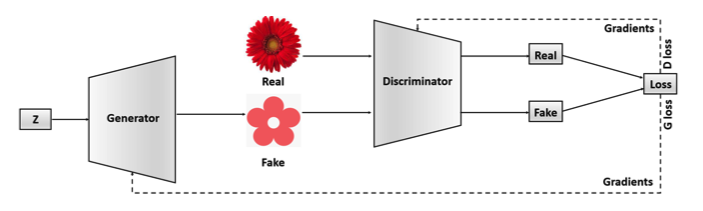
\includegraphics[width=1\linewidth]{classicalgan.png}
    \caption{Illustration of classical GAN architecture.}
    \label{fig:classical_gan}
\end{figure*}

The original GAN formulation by Goodfellow et al. (2014) introduced several key innovations \cite{goodfellow2014generativeadversarialnetworks}: Adversarial training paradigm, Non-cooperative game theory framework, Gradient-based optimization for both networks

\textbf{Training Challenges:}

As discussed in Section~2.1, classical GANs face training instability, mode collapse,
and difficulty with complex multimodal distributions when applied to bioprocess data
\cite{Arjovsky2017, gulrajani2017improved}. These challenges motivate the quantum-enhanced
approach developed in this work.

Specific challenges include:
\begin{itemize}[nosep, leftmargin=*]
  \item \textbf{Mode collapse:} Generator produces limited diversity~\cite{Arjovsky2017}
  \item \textbf{Vanishing gradients:} Discriminator becomes too strong~\cite{goodfellow2014generativeadversarialnetworks}
  \item \textbf{Hyperparameter sensitivity:} Learning rates, batch sizes critically affect convergence~\cite{gulrajani2017improved}
\end{itemize}

\subsubsection{Wasserstein Distance Mathematical Derivation}

The Wasserstein distance, also known as the Earth Mover's Distance (EMD), provides a principled way to measure the dissimilarity between two probability distributions. \cite{villani2008optimal} For two probability measures $\mu $ and $\nu$ on a metric space M with distance function d:
\begin{equation}
    W_p(\mu, \nu) = \left(\inf_{\gamma \in \Gamma(\mu,\nu)} \int_{M \times M} d(x,y)^p d\gamma(x,y)\right)^{1/p}
\end{equation}


where $\Gamma(\mu, \nu)$ denotes the set of all joint probability measures on $M \times M$ with marginals $\mu$ and $\nu$.

\textbf{Kantorovich-Rubinstein Duality:}

For $p=1$, the Wasserstein distance can be expressed as:
\begin{equation}
W_1(\mu, \nu) = \sup_{\|f\|_L \leq 1} \left|\int f d\mu - \int f d\nu\right|
\end{equation}
where the supremum is over all 1-Lipschitz functions.

This formulation allows WGAN to use a neural network (the critic) to approximate the supremum, leading to the practical WGAN objective. \cite{arjovsky17a} The Wasserstein GAN (WGAN) was introduced to address training instabilities by using the Earth Mover's distance to provide a more meaningful and stable loss metric. \cite{arjovsky17a}  The WGAN-GP further refined this approach by replacing weight clipping with a soft gradient constraint. \cite{gulrajani2017improved}

\subsubsection{Quantum Computing Fundamentals for QGANs}

\textbf{Quantum State Representation:}

A quantum state of n qubits is represented by a vector in a $2^n$-dimensional Hilbert space:

$$|\psi\rangle = \sum_{i=0}^{2^n-1} \alpha_i |i\rangle$$

where $\sum_i |\alpha_i|^2 = 1$ (normalization condition).



\textbf{Key Quantum Gates Used:}
\begin{itemize}[nosep, leftmargin=*]
  \item \textbf{Hadamard ($H$):} Creates superposition: $H\ket{0} = \frac{1}{\sqrt{2}}(\ket{0} + \ket{1})$
  \item \textbf{Rotation gates ($R_x$, $R_y$, $R_z$):} Parameterized single-qubit rotations
  \item \textbf{CNOT:} Two-qubit entangling gate
\end{itemize}

\textbf{Quantum Advantage for Generative Models:}

QGANs leverage the inherent properties of quantum systems to provide potential advantages over classical generative models. \cite{Dallaire_Demers_2018, Lloyd_2018, Zoufal_2019}

Specific advantages include:
\begin{itemize}[nosep, leftmargin=*]
  \item \textbf{Exponential state space:} $n$ qubits represent $2^n$ amplitudes, enabling more efficient representation of complex probability distributions \cite{zoufal2021generativequantummachinelearning}
  \item \textbf{Quantum interference:} Constructive/destructive interference explores solution space more efficiently
  \item \textbf{Entanglement:} Creates correlations impossible in classical probability, potentially affecting convergence behaviour; we do not claim a mode-collapse advantage and did not measure one  \cite{romero2019variationalquantumgeneratorsgenerative, Amin_2018}
\end{itemize}

Quantum interference effects can enhance the model's ability to capture subtle correlations and nonlinear relationships present in real-world data, making them particularly suited for complex temporal dependencies found in bioprocess systems. Practical scalability nonetheless remains constrained by current NISQ-device noise and limited circuit depth \cite{Cerezo_2021}.  % [55]-[57],[59] (VQE / option-pricing / QAOA / adversarial-robustness) removed: they do not support a quantum-advantage-for-bioprocess-generation claim (R1-m1)

Recent experimental implementations have demonstrated proof-of-concept QGANs on noisy intermediate-scale quantum (NISQ) devices.  \cite{rudolph2022generationhighresolutionhandwrittendigits, Huang_2021} Rudolph et al. demonstrated that QGANs can generate high-resolution images using an ion trap quantum computer, highlighting the potential of quantum models to exceed classical limitations in certain generative tasks. \cite{rudolph2022generationhighresolutionhandwrittendigits}

\subsection{Proposed Extension (Outlook): Hybrid-GAN-Mechanistic Framework}

\subsubsection{Proposed Mathematical Formulation (not implemented in this study)}

\emph{The following Hybrid-GAN-mechanistic structure is a proposed extension and was not implemented, trained, or evaluated in this work; it is included to motivate future research and is presented as a formulation only.} The proposed Hybrid-GAN-mechanistic structure would integrate generative adversarial networks with physics-informed mechanistic components to enhance predictive modeling in data-scarce environments. This approach complements hybrid machine learning approaches prevalent in chemical and biological process modeling applications, particularly when data availability is limited.  \cite{mansouri2025models, nielsen2020hybrid,nazemzadeh2021integration, ehtesham2025dynamics}

\begin{figure*}
    \centering
    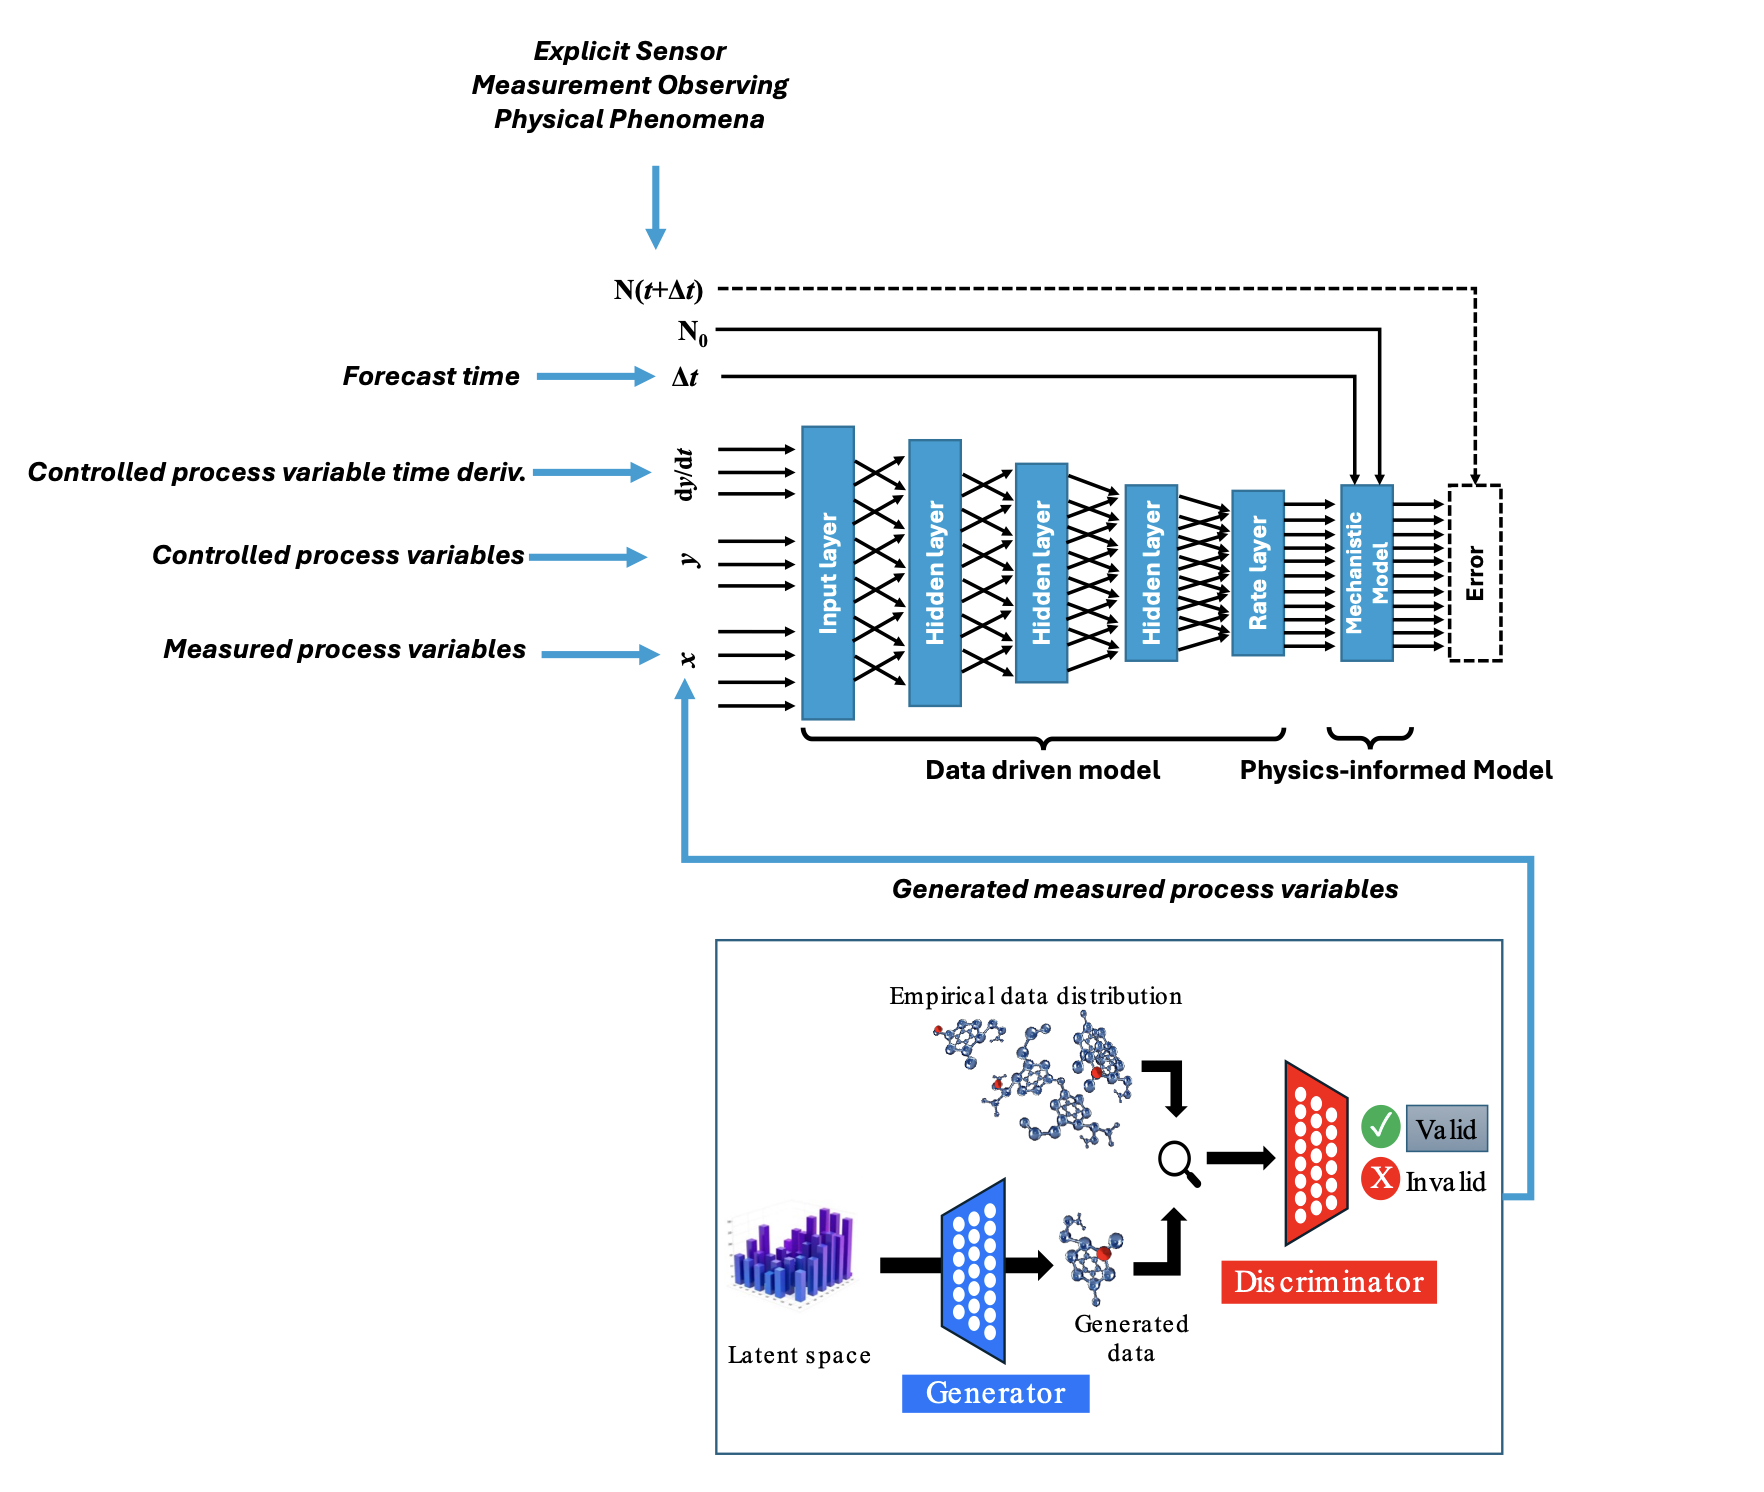
\includegraphics[width=1\linewidth]{hybridgan.png}
    \caption{QGAN and synthetic data implementation within a hybrid-model approach to process monitoring.}\label{fig:qgan_hybrid_approach}
\end{figure*}

Hybrid modeling typically combines parametric models derived from first-principles knowledge such as reaction kinetics or mass balances with nonparametric, data-driven techniques like neural networks to mitigate the challenges of sparse datasets. \cite{sharma2022hybrid} For example, hybrid models augment mechanistic simulations with machine learning to improve accuracy in bioprocessing, where experimental data are often costly and scarce due to lack of process analytical technology (PAT) or regulatory restrictions (especially in biopharmaceutical production processes), enabling reliable predictions for process optimization and control.\cite{O'Brien2021A}

The Hybrid-GAN structure integrates GANs with physics-informed mechanistic components:

\begin{equation}
\begin{split}
\min_G \max_D \bigl[ & \mathbb{E}_{x\sim p_{data}}[\log D(x)] \\
& + \mathbb{E}_{z\sim p_z}[\log(1-D(G(z)))] \\
& + \lambda\mathbb{E}_{z\sim p_z}\biggl[\biggl\|\frac{d}{dt}M(G(z)) \\
& \qquad - f(M(G(z)), t, \theta)\biggr\|^2\biggr] \bigr]
\end{split}
\end{equation}

\paragraph{Relationship to the trained objective.} The objective above is
written in the original (log-GAN / Jensen--Shannon) form,
$\mathbb{E}[\log D(x)] + \mathbb{E}[\log(1-D(G(z)))]$, augmented with a
mechanistic-residual penalty. This is deliberately distinct from the objective
actually trained in this study, which is the Wasserstein GAN with gradient
penalty (Eq.~\ref{eq:wgangp}, Earth-Mover formulation). The log-GAN form is
retained here only because it most transparently exposes where a mechanistic
residual term would attach; any future implementation of this proposed
extension would substitute the Wasserstein--gradient-penalty critic used
throughout the present work (Section~3) for the $\log D$ discriminator, so that
the Hybrid-GAN inherits the training stability documented for the deployed
QWGAN-GP rather than the mode-collapse and vanishing-gradient pathologies of
the original GAN objective.

\textbf{Components:}
\begin{itemize}[nosep, leftmargin=*]
  \item $G$: Generator mapping latent variables $z$ to generated process variables
  \item $D$: Discriminator assessing authenticity
  \item $M$: Mechanistic operator projecting generated data onto physical states
  \item $f$: Governing dynamics (e.g., ODEs describing bioprocess kinetics)
  \item $\lambda$: Weighting hyperparameter balancing data fidelity and physical consistency
  \item $\theta$: Model parameters from constitutive equations (reaction kinetics, particle size distribution, growth rates, etc.)
\end{itemize}

This optimization balances statistical fidelity from empirical data distributions ($p_{data}$) with physical consistency, minimizing residuals from time derivatives.

\subsubsection{Integration with Process Models}


\begin{figure}[ht]
  \centering
  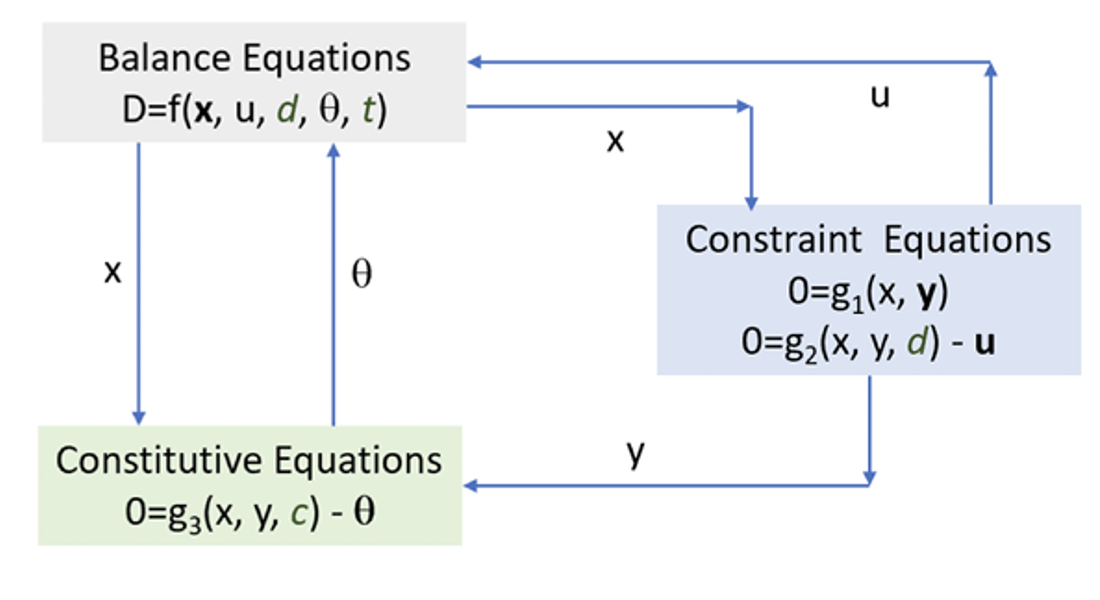
\includegraphics[width=\columnwidth]{mech_rep.png}
  \caption{Mechanistic representation of (bio)chemical processes. Reprinted with permission from Elsevier. \cite{mansouri2025models}}
  \label{fig:mech_rep}
\end{figure}

The mechanistic representation involves several key equation types:

\textbf{Balance Equations:}
\begin{equation}
  D = f(x, u, d, \theta, t)
  \label{eq:balance}
\end{equation}

\textbf{Constraint Equations:}
\begin{align}
  0 &= g_1(x, y) \label{eq:constraint1} \\
  0 &= g_2(x, y, d) - u \label{eq:constraint2}
\end{align}

\textbf{Constitutive Equations:}
\begin{equation}
  0 = g_3(x, y, c) - \theta
  \label{eq:constitutive}
\end{equation}

\noindent where:
\begin{itemize}[nosep, leftmargin=*]
  \item $c$: vector of model parameters
  \item $d$: vector of specified variables
  \item $t$: independent variable (time)
  \item $u$: vector of design variables
  \item $x$: vector of process variables
  \item $y$: vector of measured variables
  \item $\theta$: vector of physico-chemical properties
\end{itemize}

This structure extends physics-informed neural networks (PINNs) paradigm by incorporating adversarial training for synthetic data augmentation in data-limited scenarios. This connection underscores the Hybrid-GAN's utility in addressing small data challenges, where pure data-driven models fail due to insufficient training samples, by infusing prior scientific knowledge to produce robust, generalizable predictive models.

\subsubsection{Comparison with Other Modeling Approaches}

\begin{table}
\small
\caption{\emph{Qualitative, aspirational} comparison of modelling approaches in data-scarce environments. The ratings are conceptual expectations from the literature, \emph{not} measured outcomes of this study; in particular the ``Hybrid-GAN (Proposed)'' row describes a proposed architecture that was not implemented or evaluated here.}
\label{tbl:various_approaches}
\resizebox{\columnwidth}{!}{%
\begin{tabular}{p{2cm}p{2cm}p{2cm}p{2cm}p{2.55cm}p{2cm}}
\hline
\textbf{Method} & \textbf{Data Efficiency} & \textbf{Physical Consistency} & \textbf{Generative Capability} & \textbf{Interpretability} & \textbf{Robust to Small Data}\\
\hline
Pure Data-Driven Models & \textbf{\ding{55}}& \textbf{\ding{55}}& \textbf{\ding{51}}& \textbf{\ding{55}}& \textbf{\ding{55}} \\
\midrule
Mechanistic Models & \textbf{\ding{51}}& \textbf{\ding{51}}& \textbf{\ding{55}}& \textbf{\ding{51}}& \textbf{\ding{51}}\\
\midrule
Hybrid Models (Mech + ML) & \textbf{\ding{51}}& \textbf{\ding{51}}& \textbf{\ding{55}}& \textbf{\ding{51}}& \textbf{\ding{51}}\\
\midrule
PINNs & \textbf{\ding{51}}& \textbf{\ding{51}}& \textbf{\ding{55}}& \textbf{\ding{51}}& \textbf{\ding{51}}\\
\midrule
Standard GANs & \textbf{\ding{55}}& \textbf{\ding{55}}& \textbf{\ding{51}}& \textbf{\ding{55}}& \textbf{\ding{55}}\\
\midrule
Hybrid-GAN (Proposed) & \textbf{\ding{51}}& \textbf{\ding{51}}& \textbf{\ding{51}}& \textbf{\ding{51}}& \textbf{\ding{51}} \\
\bottomrule
\end{tabular}}
%}
\end{table}

This table is an \emph{aspirational} qualitative comparison: the ``Hybrid-GAN (Proposed)'' row reflects expected properties of the proposed extension and was \emph{not} experimentally validated in this study. It is provided to motivate future work, not as a demonstrated result. If a measured comparison cannot be provided, the row (or the table) may be removed at the editor's discretion.

\subsubsection{Expected Regularization Properties}

In principle, the physics term $M(G(z))$ would impose mechanistic constraints that reduce overfitting \cite{rice2020overfittingadversariallyrobustdeep}, while sensor measurements ($y$) would constrain the latent space to physically feasible dynamics \cite{hermann2025hybrid}. These properties remain to be validated empirically.


\subsection{Additional Validation Metrics Discussion} 

\subsubsection{Dynamic Time Warping (DTW) Implementation}

Dynamic Time Warping (DTW) represents a powerful technique for measuring similarity between temporal sequences that may exhibit varying lengths or temporal misalignments. \cite{dimoudis2023utilizing} The DTW algorithm operates by identifying an optimal warping path that minimizes the cumulative distance between corresponding elements of two time series while respecting monotonicity and boundary constraints.

\begin{algorithm}[ht]
  \caption{Dynamic Time Warping}
  \label{alg:dtw}
  \begin{algorithmic}[1]
    \Require Time series $S$ of length $n$, time series $T$ of length $m$
    \Ensure DTW distance between $S$ and $T$
    \State $\mathbf{DTW} \gets (n+1) \times (m+1)$ matrix
    \State $\mathbf{DTW}[0,\,0] \gets 0$
    \For{$i = 1$ to $n$}
      \State $\mathbf{DTW}[i,\,0] \gets \infty$
    \EndFor
    \For{$j = 1$ to $m$}
      \State $\mathbf{DTW}[0,\,j] \gets \infty$
    \EndFor
    \For{$i = 1$ to $n$}
      \For{$j = 1$ to $m$}
        \State $\text{cost} \gets |S[i] - T[j]|$
        \State $\mathbf{DTW}[i,\,j] \gets \text{cost} + \min\begin{cases}
          \mathbf{DTW}[i-1,\,j]   & \text{insertion} \\
          \mathbf{DTW}[i,\,j-1]   & \text{deletion} \\
          \mathbf{DTW}[i-1,\,j-1] & \text{match}
        \end{cases}$
      \EndFor
    \EndFor
    \State \Return $\mathbf{DTW}[n,\,m]$
  \end{algorithmic}
\end{algorithm}

\textbf{Interpretation:}
Lower DTW scores indicate better temporal alignment. Under the matched parameter budget and matched 2000-epoch training contract, the OD-scale DTW distance for the 55-parameter IQP:SEL quantum generator is approximately 0.30 (mean over 5 seeds). A frozen pre-v1.0 best-case checkpoint reported a DTW score of 0.6843; this value is not re-emitted under the matched-budget contract and is retained here only as a historical reference. DTW is robust to phase shifts and speed variations in time series.

\paragraph{Reconciliation with the pre-v1.0 DTW reference.}
An earlier frozen pre-v1.0 best-case checkpoint reported an OD-scale DTW distance of 0.6843. That value was computed under a legacy preprocessing pipeline (Pipeline~A; not the matched-budget Pipeline~B), under a single-seed best-case selection, and at a different epoch budget. Under the matched-budget contract (Pipeline~B, 5-seed mean, 2000 epochs) reported in Section~4 of the main text, the corresponding OD-scale DTW for the 55-parameter IQP:SEL quantum generator is $0.302 \pm 0.030$; the 0.6843 figure is retained only for historical traceability and is not directly comparable to the matched-budget results.

The selection of DTW for temporal sequence comparison stems from its ability to accommodate local temporal distortions while preserving the overall sequential structure. Unlike rigid distance metrics, DTW provides robust similarity measurements for time-dependent data by dynamically adjusting for speed variations, length differences, and localized temporal shifts that commonly occur in real-world temporal patterns.


\subsection{Code and Data Availability}
Complete code repository: \url{https://github.com/shawngibford/qgan}

Archived snapshot of the tagged release: Zenodo, DOI: \texttt{ZENODO-DOI-PLACEHOLDER} (to be assigned at release-freeze time).

The complete code, trained models, and datasets have been released for transparency, independent verification, and acceleration of subsequent advances in quantum-enhanced chemical and biochemical engineering.


\textbf{Quantum Circuit Specifications:}

The quantum circuit employs a dual-stage encoding strategy as described in Section~3 of the main text:
\begin{itemize}[nosep, leftmargin=*]
  \item 5 qubits arranged in three layers
  \item IQP (Instantaneous Quantum Polynomial) encoding
  \item Strongly entangling layers with $\text{Rot}(\phi, \theta, \omega)$ gates
  \item Range-based CNOT gates: $r = (\text{layer} \bmod (n_{\text{qubits}} - 1)) + 1$
  \item Enhanced Pauli measurements ($X$ and $Z$ expectation values)
  \item Total parameters: 55 (5 for IQP encoding, 45 for the three strongly entangling layers, 5 for measurement-preparation rotations)
\end{itemize}

\subsection{Additional Figures}

\textbf{Detailed Quantum Circuit Decomposition}


\begin{figure*}
    \centering
    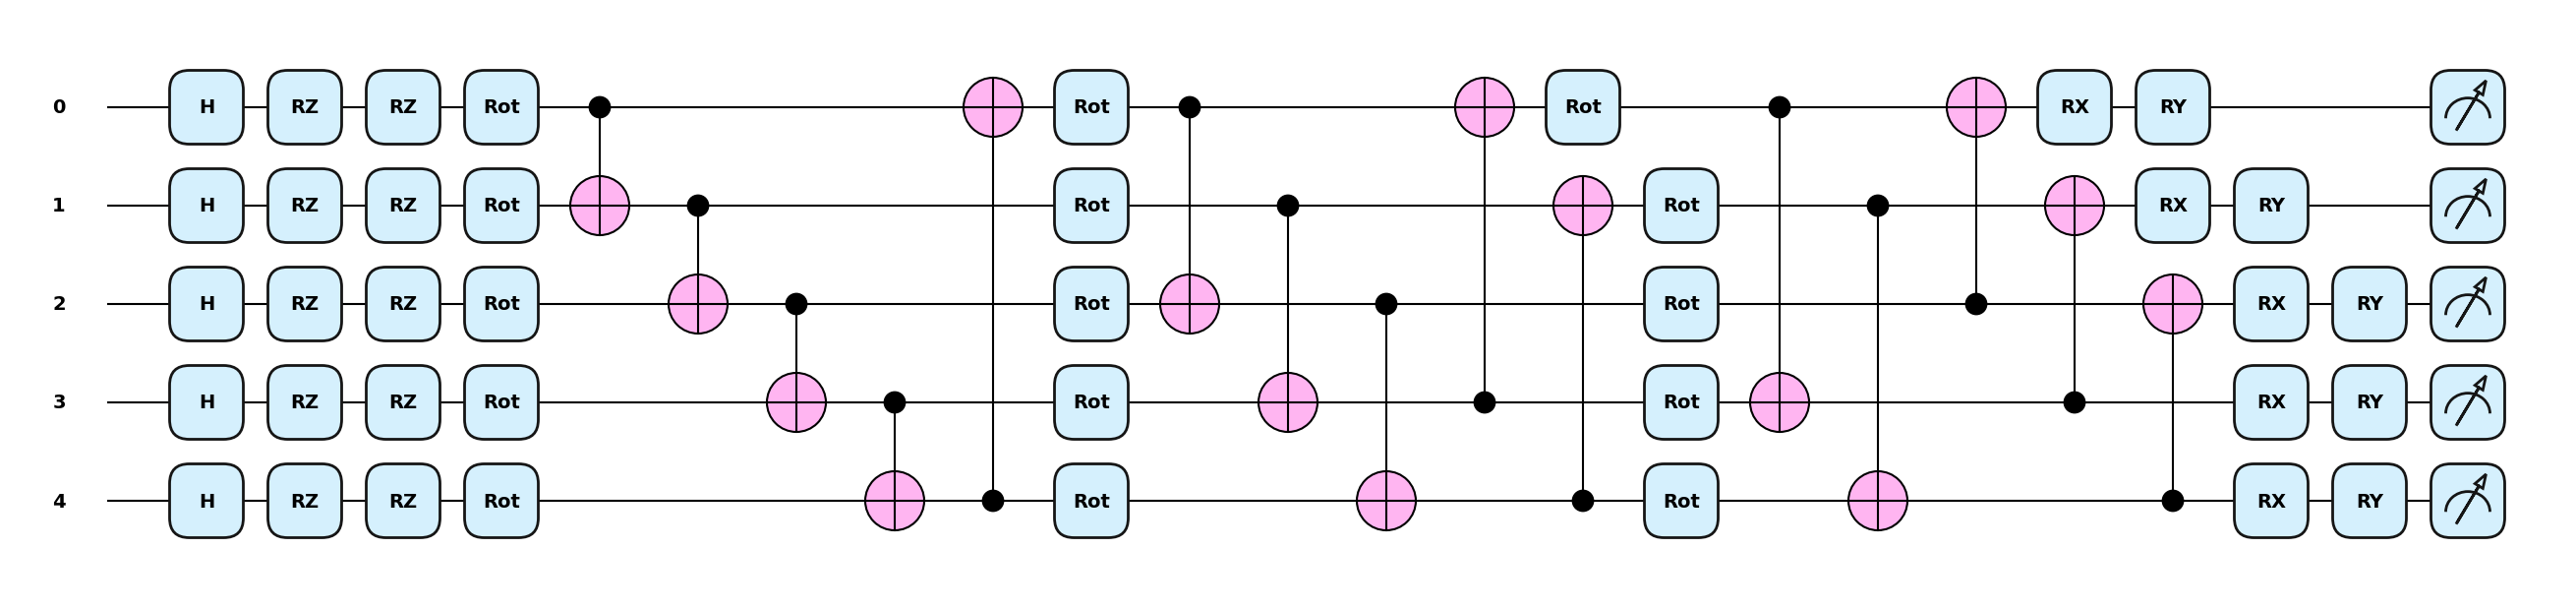
\includegraphics[height = 5cm, width=1\linewidth]{quantum_circuit.png}
    \caption{Quantum circuit used as generator.}
    \label{fig:quantum_circuit}
\end{figure*}


This figure shows the individual gate operations, including:
Hadamard gates applied to all qubits for superposition creation, 
First IQP encoding layer with Rz gates using random noise, 
Second IQP encoding layer with parameterized Rz rotations, 
Two strongly entangling layers with Rot gates and range-based CNOT gates, 
Final rotation gates (Rx and Ry) for measurement preparation, 
and Pauli-X and Pauli-Z measurements.

The circuit implements the architecture described in Section 3, leveraging quantum superposition and entanglement to explore multiple solution paths simultaneously during training, potentially affecting training dynamics (not evaluated in this study). \cite{romero2019variationalquantumgeneratorsgenerative, Amin_2018}


\begin{figure*}
    \centering
    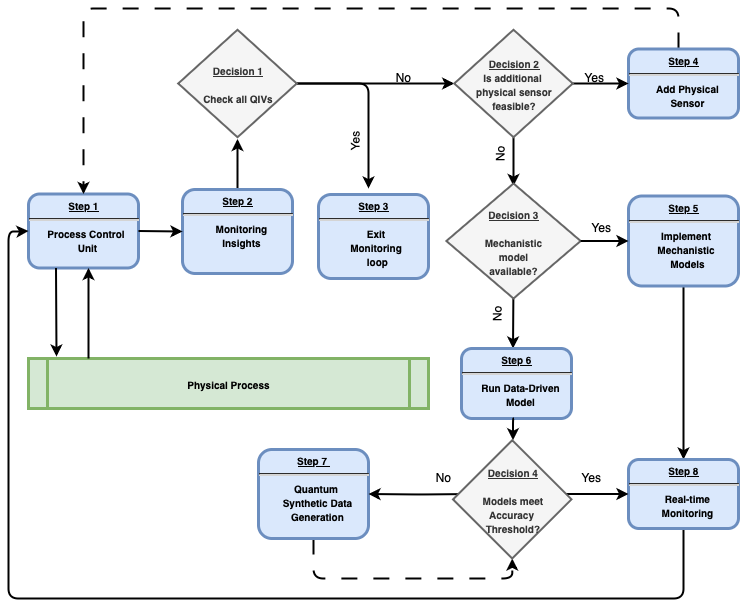
\includegraphics[width=0.75\linewidth]{bpm_qgan.drawio.png}
    \caption{Decision-tree triage schematic for bioprocess monitoring, outlined as future work in §4.5 Outlook of the main text. Not an empirical contribution of the present study.}\label{fig:qgan_schematic}
\end{figure*}
This figure illustrates the decision-tree triage workflow outlined as future work in Section~4.5 (Outlook) of the main text, sketching how sensor-feasibility, mechanistic, data-driven, and quantum-synthetic options could be organised under varying data-availability constraints. It is presented as an organising concept and is not evaluated empirically in this paper.
\begin{figure*}
    \centering
    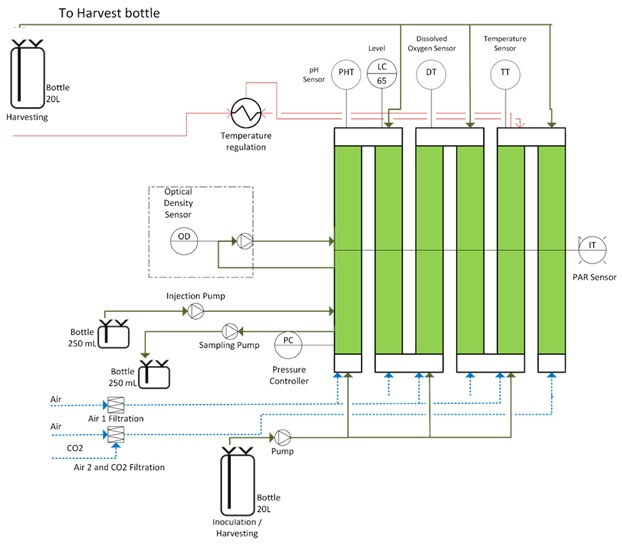
\includegraphics[width=1\linewidth]{lucy_diagram.jpg}
    \caption{Schematic of the 20\,L LUCY\textregistered{} photobioreactor used in this study, with its sensors and actuators.}
    \label{fig:lucy}
\end{figure*}

This schematic depicts the photobioreactor experimental setup described in Section~3.2, showing the sensor and actuator configuration used for data acquisition.

\subsection{Data Transformation Details}

\begin{figure}[h]
  \centering
  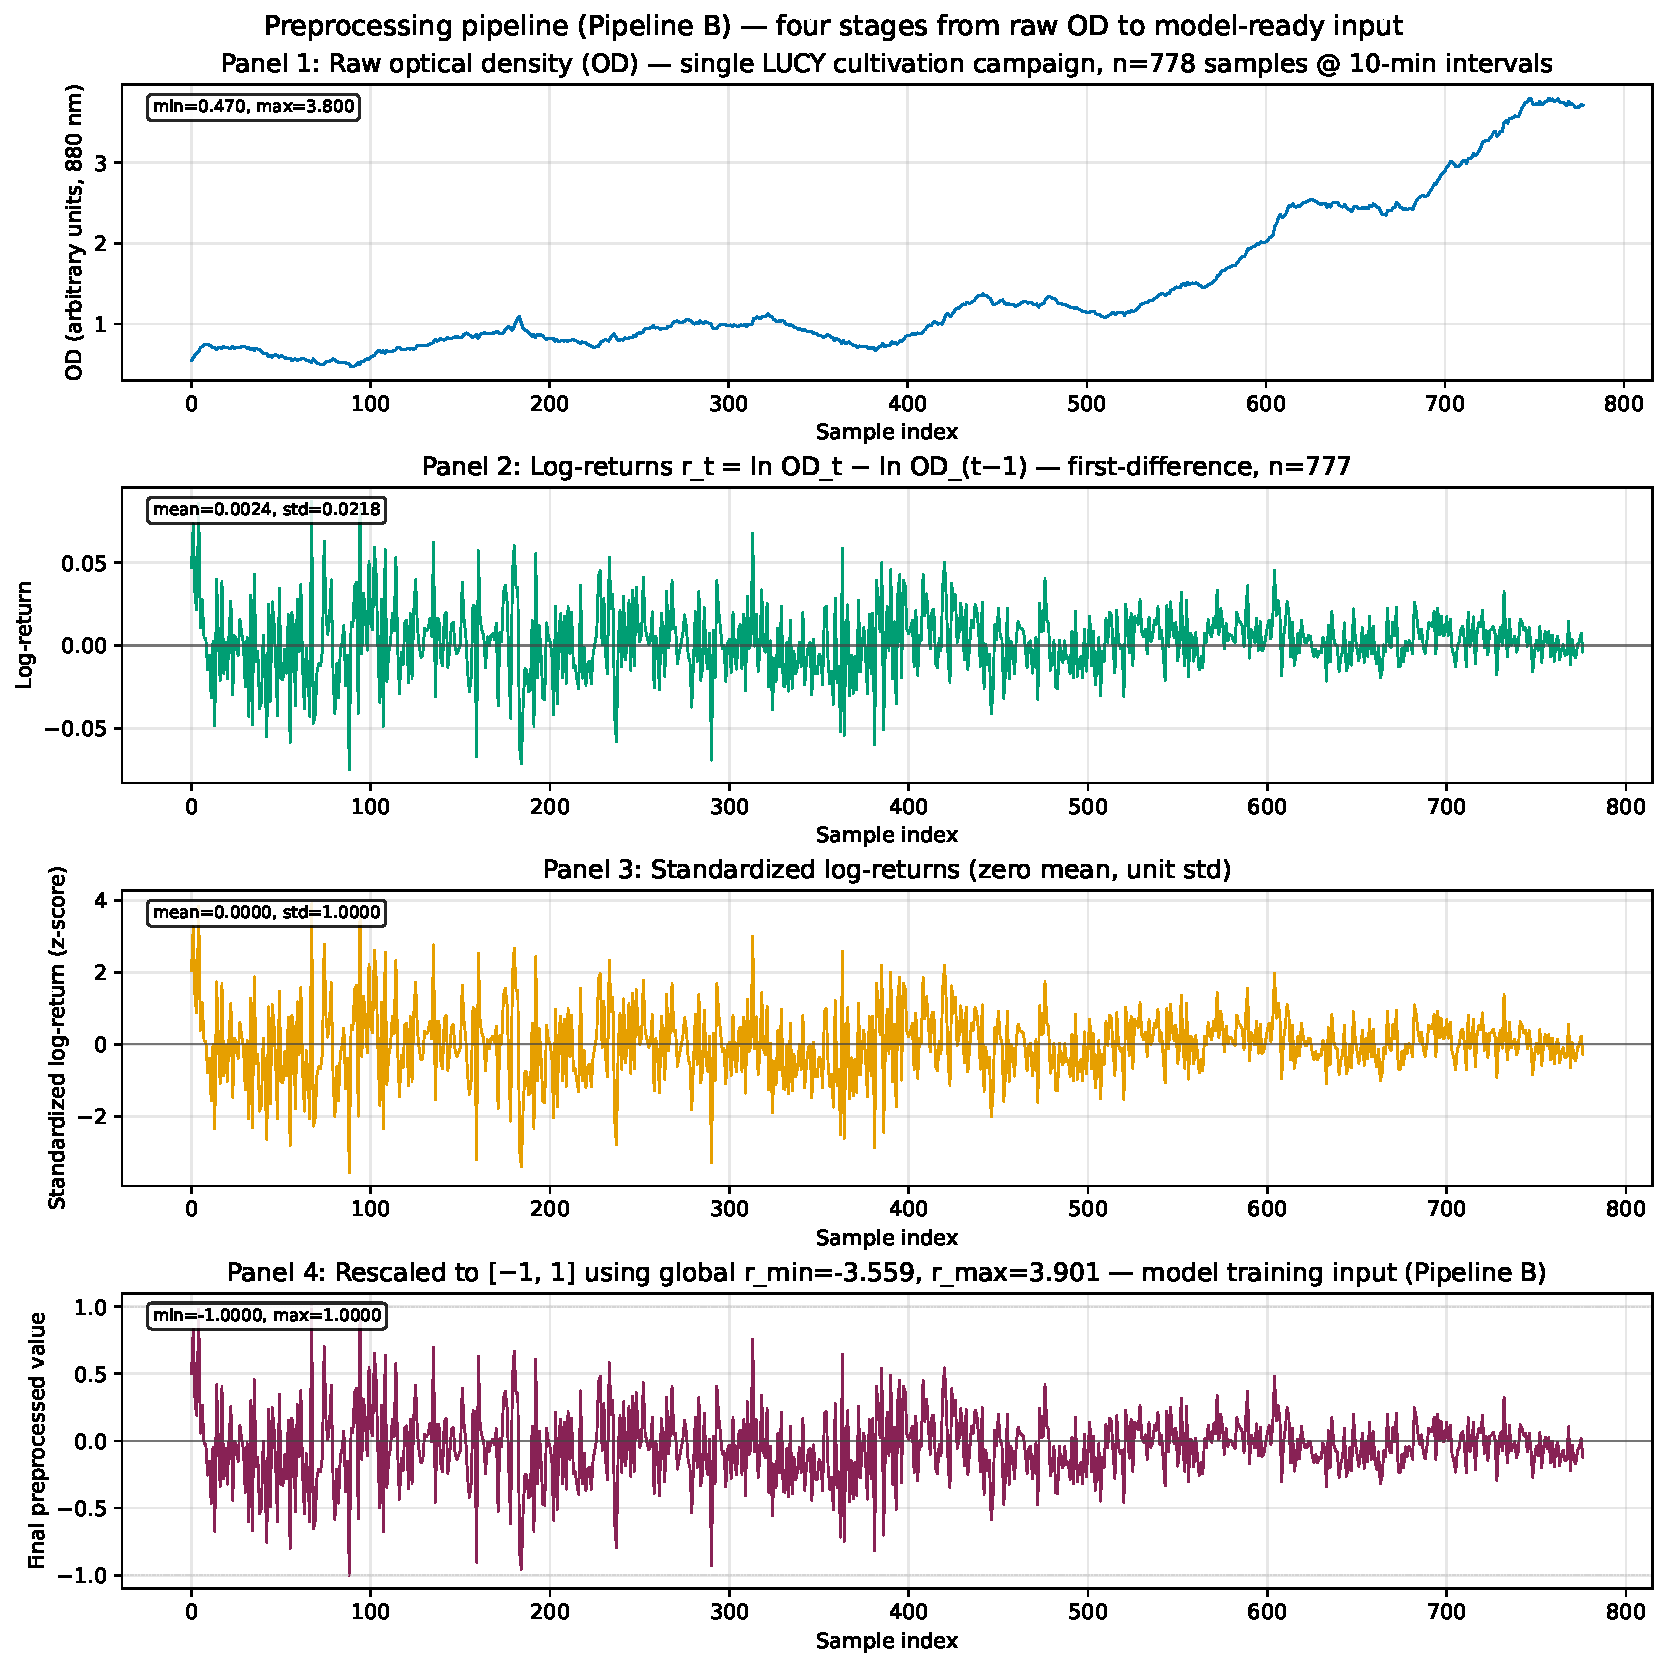
\includegraphics[width=\columnwidth]{revision/results/figures/preprocessing_pipeline_4panel.pdf}
  \caption{Four-stage preprocessing pipeline (Pipeline~B, native): raw OD ($n=778$),
  log-returns $r_t = \ln \mathrm{OD}_t - \ln \mathrm{OD}_{t-1}$ ($n=777$),
  standardized ($\mu=0$, $\sigma=1$), and inverse Lambert~$W$ heavy-tail correction
  $+$ rescale to $[-1, 1]$. The trained generators operate on the final-stage
  rescaled log-return windows; all matched-budget evaluation results in
  Section~4 of the main text are reported under this pipeline. Source:
  \texttt{revision/results/figures/preprocessing\_pipeline\_4panel.json}.}
  \label{fig:preprocessing_pipeline}
\end{figure}

The transformation from optical density measurements to log differences is motivated by the bioprocess itself: for an exponentially growing culture the optical density follows $\mathrm{OD}_t \approx \mathrm{OD}_0\,e^{\mu t}$, so the log difference between successive samples is a direct discrete estimate of the instantaneous specific growth rate. For optical density measurements $OD_t$ at time $t$:

$$r_t = \ln(\text{OD}_t) - \ln(\text{OD}_{t-1}) \;\approx\; \mu_t\,\Delta t$$

where $\mu_t$ is the local specific growth rate over the sampling interval $\Delta t$. Working in $r_t$ rather than raw OD has a direct bioprocess interpretation and three practical benefits for this growth-rate signal:
\begin{itemize}[nosep, leftmargin=*]
  \item \textbf{Growth-rate interpretability:} each $r_t$ is (up to the sampling interval) the specific growth rate, the quantity of physiological interest in cultivation monitoring, rather than an arbitrary attenuation reading
  \item \textbf{Scale/stage invariance:} the log difference is invariant to the absolute OD level, so early-exponential and high-density phases are placed on a comparable scale, which stabilises learning across the growth curve
  \item \textbf{Additivity:} growth rates over consecutive intervals sum to the net log-growth over the total span, matching how cumulative biomass increase is reported
\end{itemize}

The finance literature uses the same transform for unrelated reasons; here the justification is physiological (growth-rate estimation), not financial.

\textbf{Normalization:}
\begin{equation}
  r_t^{\,\text{NORM}} = \frac{r_t - \mu}{\sigma}
  \label{eq:normalization_s9}
\end{equation}

This brings all values to a consistent scale with mean zero and standard deviation one, which is essential for quantum circuit encoding.

\textbf{Lambert $W$ Transformation:}

The inverse Lambert $W$ transform was applied to the normalized log values to adjust for heavy tails within the distribution of the data, pushing them towards more Gaussian traits. As shown by Goerg~\cite{goerg2015lambert}, this function allows the reshaping of a distribution to align more closely with a Gaussian distribution:
\begin{equation}
  W_\delta(\nu) = \text{sgn}(\nu)\sqrt{\frac{W(\delta\nu^2)}{\delta}}
  \label{eq:lambert_w_s9}
\end{equation}

\noindent where:
\begin{itemize}[nosep, leftmargin=*]
  \item $\nu$ is a value of the dataset
  \item $\text{sgn}(\nu)$ is the sign of $\nu$
  \item $\delta$ is a programmable parameter
  \item $W$ is the Lambert $W$ function (inverse of $z = ue^u$)
\end{itemize}

This transformation is particularly important for bioprocess data, which often exhibits non-normal distributional properties due to the inherent variability and complex underlying mechanisms~\cite{boskabadi2025virtual}.

\subsubsection{Rolling Window Implementation}

Using the rolling window technique~\cite{dimoudis2023utilizing}, we generated overlapping subsequences of the original data to capture temporal patterns and dependencies. This depends on two parameters:
\begin{itemize}[nosep, leftmargin=*]
  \item \textbf{Stride ($s$):} The gap between the starts of subsequences (set to 2)
  \item \textbf{Subsequence length ($m$):} The length of each window (set to 10)
\end{itemize}

The window length ($m$) is set longer than ($s$) to guarantee enough overlap. According to Orlandi et al.~\cite{orlandi2024enhancing}, these values optimize for balanced overlap and computational efficiency. This approach is essential for capturing the temporal dependencies that characterize bioprocess dynamics, where events at one time point influence future states.

\subsection{Critic Network Architecture Details}

The Critic model is a convolutional neural network that processes sequential data to distinguish between real and generated data from the quantum generator. The network follows the WGAN-GP architecture~\cite{gulrajani2017improved} with specific adaptations for time series data.

% source: revision/results/total_adversarial_param_budget.json#shared_critic_n_params (=250881)
% source: revision/results/classical_architectures.json#models.shared_critic.total_params (=250881)
The critic network has a total of 250881 trainable parameters. This same
critic was used for all WGAN-GP generators (quantum and classical) under the
matched-budget protocol defined in main-text Section~3.1; the only component
that varies between the quantum and classical entrants is the generator,
which isolates the effect of the quantum circuit on the generated
distribution.

\textbf{Architecture Specifications:}

\textbf{Convolutional Layers:}
\begin{itemize}[nosep, leftmargin=*]
  \item Layer 1: 64 filters, kernel size 3, stride 1
  \item Layer 2: 128 filters, kernel size 3, stride 1
  \item Layer 3: 128 filters, kernel size 3, stride 1
\end{itemize}

The increasing filter count allows extraction of more complex features and produces detailed feature maps. The first convolutional layer is designed to handle input data shaped as $(10, 1)$, where the dimension of 10 represents the length of subsequences created through the rolling window approach~\cite{dimoudis2023utilizing}, ensuring the network properly processes the temporal structure of the input data.

\textbf{Activation Functions:}

Each convolutional layer is followed by a LeakyReLU activation function ($\alpha = 0.1$), which addresses the vanishing gradient issue that can cause neurons to become inactive and enables the network to learn more complex patterns through its nonlinear properties~\cite{gulrajani2017improved}.

\textbf{Dense Layers:}

Following the three convolutional layers, the data undergoes flattening to convert the multidimensional feature maps into a one-dimensional vector suitable for dense layer processing. A fully connected layer with 32 neurons is then applied with LeakyReLU activation to capture complex data relationships.

\textbf{Regularization:}

To improve generalization and reduce overfitting, a dropout layer randomly deactivates 20\% of neurons during training.

\textbf{Output Layer:}

The final output layer contains a single neuron that produces an unbounded scalar value, where higher values indicate the input resembles real data and lower values suggest generated data. This unbounded output design aligns with the use of Wasserstein distance as the cost function~\cite{arjovsky17a}, providing more meaningful gradients during training compared to the original GAN formulation~\cite{goodfellow2014generativeadversarialnetworks}.





\end{document}

